
% *** Authors should verify (and, if needed, correct) their LaTeX system  ***
% *** with the testflow diagnostic prior to trusting their LaTeX platform ***
% *** with production work. IEEE's font choices can trigger bugs that do  ***
% *** not appear when using other class files.                            ***
% The testflow support page is at:
% http://www.michaelshell.org/tex/testflow/

\documentclass[conference]{IEEEtran}
\usepackage[latin1]{inputenc}
\usepackage{subfigure}
\usepackage{amsmath}
\usepackage{amssymb}
\usepackage[ruled,lined,linesnumbered,longend]{algorithm2e}
% Add the compsoc option for Computer Society conferences.
%
% If IEEEtran.cls has not been installed into the LaTeX system files,
% manually specify the path to it like:
% \documentclass[conference]{../sty/IEEEtran}

% *** CITATION PACKAGES ***
%
\usepackage{cite}

% *** GRAPHICS RELATED PACKAGES ***
%
\ifCLASSINFOpdf
\usepackage[pdftex]{graphicx}
  % declare the path(s) where your graphic files are
\graphicspath{{./pdf/}{./jpeg/}}
  % and their extensions so you won't have to specify these with
  % every instance of \includegraphics
   \DeclareGraphicsExtensions{.pdf,.jpeg,.png}
\else
  % or other class option (dvipsone, dvipdf, if not using dvips). graphicx
  % will default to the driver specified in the system graphics.cfg if no
  % driver is specified.
  \usepackage[dvips]{graphicx}
  % declare the path(s) where your graphic files are
  \graphicspath{{../eps/}}
  % and their extensions so you won't have to specify these with
  % every instance of \includegraphics
  \DeclareGraphicsExtensions{.eps}
\fi


\usepackage{stfloats}

% *** PDF, URL AND HYPERLINK PACKAGES ***
%
\usepackage{url}

% correct bad hyphenation here
\hyphenation{op-tical net-works semi-conduc-tor}

\begin{document}
%
% paper title
% can use linebreaks \\ within to get better formatting as desired
\title{Fiding scalable evolutionary solutions to the game of MasterMind}

% author names and affiliations
% use a multiple column layout for up to three different
% affiliations
\author{\IEEEauthorblockN{Juan-J. Merelo,  Antonio M. Mora \\ and Pedro A. Castillo}
\IEEEauthorblockA{Departamento de Arquitectura y Tecnolog\'ia de Computadores \\
University of Granada\\
Email: \{jmerelo,amorag,pedro\}@geneura.ugr.es}
\and
\IEEEauthorblockN{Carlos Cotta}
\IEEEauthorblockA{Departamento de Lenguajes y Ciencias de la Computaci\'on\\
Universidad de M\'alaga\\
Email: ccottap@lcc.uma.es}
\and
\IEEEauthorblockN{Mario Valdez}
\IEEEauthorblockA{Instituto Tecnol\'ogico de Tijuana\\
Tijuana, M\'exico\\
Email: mario@tectijuana.edu.mx}
}

% make the title area
\maketitle

\begin{abstract}
MasterMind is a puzzle in which a hidden string of symbols must be
discovered by producing query strings which are compared with the
hidden one; the result of this comparison (in terms of {\em number}
of correct positions and colors) is fed back to the
player that is trying to crack the code (codebreaker).
% Antonio - en lugar de discoverer -> enquirer o algo asÌ?
Methods for solving this puzzle 
% Antonio - DÛnde? En la literatura? Usually?
are usually compared in terms of the number of query strings (guesses) made and the total time needed to produce those strings. In this paper we focus on the latter by trying 
% Antonio - by trying -> trying?
% no, est· bien - JJ
to find a combination of parameters that is, first, uniform and
independent of the problem size, and second, adequate to find a fast
solution that is, at the same time, good enough. The key to this combination of parameters
% Antonio - acabas de decir que era una combinaciÛn de par·metros
% OK
will be the {\em consistent set size}, that is, the maximum number of
combinations that are sought before being scored and played as a
guess. Having found in previous papers that the size has an influence
on speed, we will concentrate on small sizes and test them through two
different scoring methods from literature: most parts and entropy
% Antonio - quÈ se quiere demostrar? quÈ se ha demostrado finalmente?
to find out the influence of that parameter on the outcome and which
method scales better. 
\end{abstract}

\IEEEpeerreviewmaketitle

\section{Introduction and state of the art}

MasterMind \cite{Knuth,Montgomery} 
% Antonio - con una o dos refs bastarÌa, no?
is a puzzle in which one player $A$ hides a combination of
$\kappa$ symbols and length $\ell$, while the other player $B$, called
the {\em codebreaker}, tries to
uncover it by playing combinations coded in the same alphabet and with the same
length. The answers from player $A$ to every combination include the number of
symbols in the combination that are in the correct position (usually
white pins) and the number of colors that have been guessed correctly
(black pins).  
% Antonio - corrÌgeme si me he equivocado con los colores de las pistas. :D
Player $B$ then plays new combinations until the hidden one is
found. The objective of the game is to play repeatedly minimizing the
number of turns needed to find the solution.  

Solving a puzzle is a challenge by itself, even if it is a lowly board
game such as this one. In fact, it is a game in which almost any
computer strategy can beat a human, who uses a very different
strategy \cite{laughlin1982selection,hubalovsky2012modeling} to play
it, namely, trying to first get the colors right and then fix the
positions (but more elaborated versions of this one are also
possible. 
% Antonio - puedes comentar en una frase quÈ estrategias usamos los
% humanos
% done - JJ
But solutions to MasterMind can be applied easily to other games such as MineSweeper \cite{legendre2012minesweeper} or Hangman since the structure is the
same: probing a part of the search space and getting a response from
whoever holds the secret. We could stop at that and call MasterMind a
worthwhile challenge, 
% Antonio - esta expresiÛn suena muy informal...
% pero mola, eh? - JJ
but it so happens that solving MasterMind can also be used to break ATMs guessing PINs \cite{focardi2011guessing} and even for an operation in biotechnology called {\em selective phenotyping} \cite{gagneur2011selective}. Not only that, but since it is a problem which is NP-Hard
\cite{DBLP:journals/corr/abs-1111-6922} the issue of finding bounds to
the number of guesses needed is still open
\cite{doerr2012playing}. Therefore, there is room for making new
venues into finding better or faster solutions to the game of
% Antonio - better es lo mismo que faster en este problema, øno?
% No necesariamente, se pueden encontrar mejores soluciones m·s
% lentamente - JJ
MasterMind such as the heuristic solution we present in this paper. 

\begin{table*}[bht]
% IdÈntico a otro trabajo publicado, cambiar si se puede
% Antonio - pos eso mismo. XD
\caption{Scheme of partitions after two combinations have been played
  in an imaginary game  after two combinations have already been
  played.  Every combination is matched with all
  the rest of the consistent set (that is, the set of consistent combinations).
% Antonio - se repite esta misma frase al principio del caption, escrÌbelo de otra forma
In boldface, the combinations which have the minimal worst set score (which 
% Antonio - no has dicho lo que es el worst set size
happens to be in the 1b-1w column, 
% Antonio - no has dicho antes quÈ es black (b) y quÈ es white (w). Yo lo he aclarado en dos parÈntesis, pero revÌsalo. ;)
but it could be any one); in this case, equal to ten. A strategy that
tries to minimize worst case would play one of those combinations. On
the other hand, the Entropy and Most Parts scores used in this paper are in the last
column; combinations with the maximum scores are {\em
  italiziced}. I this case, the strings with max score are the same.
The column 0b-1w with all values equal to 0 has been suppressed;
column for combination 3b-1w, being impossible, is not shown
either. Some rows have also been eliminated to save space.  \label{tab:partitions}}
% Antonio - ahora no hay lack of space, jeje
% cambiado - JJ
\small
\centering
\begin{tabular}{|l|c|c|c|c|c|c|c|c|c|c|l|l|}
\hline
Combination & \multicolumn{10}{|c|}{Number of combinations in the
  partition with response} & Entropy & Most Parts \\
\hline
 &0b-2w& 0b-3w& 0b-4w& 1b-1w& 1b-2w& 1b-3w& 2b-0w& 2b-1w& 2b-2w& 3b-0w
 & Score & Score \\
AABA &0 &0 &0 &14 &8 &0 &13 &1 &0 &3  & 1.350 & 5 \\
{\bf AACC} &8 &0 &0 &10 &5 &0 &8 &4 &1 &3  & 1.787 & 7 \\
AACD &6 &2 &0 &11 &6 &1 &4 &5 &1 &3  & 1.967 & 9 \\
AACE &6 &2 &0 &11 &6 &1 &4 &5 &1 &3  & 1.967 & 9 \\
AACF &6 &2 &0 &11 &6 &1 &4 &5 &1 &3  & 1.967 & 9 \\
{\bf ABAB} &8 &0 &0 &10 &5 &0 &8 &4 &1 &3  & 1.787 & 7 \\
ABAD &6 &2 &0 &11 &6 &1 &4 &5 &1 &3  & 1.967 & 9 \\
ABAE &6 &2 &0 &11 &6 &1 &4 &5 &1 &3  & 1.967 & 9 \\
ABAF &6 &2 &0 &11 &6 &1 &4 &5 &1 &3  & 1.967 & 9 \\
{\bf ABBC} &4 &4 &0 &10 &8 &0 &8 &1 &1 &3  & 1.851 & 8 \\
\textit{ ABDC  }&3 &4 &1 &11 &9 &1 &4 &2 &1 &3  & 1.991 & 10 \\
\textit{ ABEC  }&3 &4 &1 &11 &9 &1 &4 &2 &1 &3  & 1.991 & 10 \\
\textit{ ABFC  }&3 &4 &1 &11 &9 &1 &4 &2 &1 &3  & 1.991 & 10 \\
ACAA &0 &0 &0 &14 &8 &0 &13 &1 &0 &3  & 1.350 & 5 \\
{\bf ACCB} &4 &4 &0 &10 &8 &0 &8 &1 &1 &3  & 1.851 & 8 \\
ACDA &0 &0 &0 &16 &10 &2 &5 &3 &0 &3  & 1.525 & 6 \\
{\bf BBAA} &8 &0 &0 &10 &5 &0 &8 &4 &1 &3  & 1.787 & 7 \\
{\bf BCCA} &4 &4 &0 &10 &8 &0 &8 &1 &1 &3  & 1.851 & 8 \\
\textit{ BDCA  }&3 &4 &1 &11 &9 &1 &4 &2 &1 &3  & 1.991 & 10 \\
\textit{ BECA  }&3 &4 &1 &11 &9 &1 &4 &2 &1 &3  & 1.991 & 10 \\
\textit{ BFCA  }&3 &4 &1 &11 &9 &1 &4 &2 &1 &3  & 1.991 & 10 \\
{\bf CACA} &8 &0 &0 &10 &5 &0 &8 &4 &1 &3  & 1.787 & 7 \\
{\bf CBBA} &4 &4 &0 &10 &8 &0 &8 &1 &1 &3  & 1.851 & 8 \\
\textit{ CBDA  }&3 &4 &1 &11 &9 &1 &4 &2 &1 &3  & 1.991 & 10 \\
\textit{ CBEA  }&3 &4 &1 &11 &9 &1 &4 &2 &1 &3  & 1.991 & 10 \\
\textit{ CBFA  }&3 &4 &1 &11 &9 &1 &4 &2 &1 &3  & 1.991 & 10 \\
DACA &6 &2 &0 &11 &6 &1 &4 &5 &1 &3  & 1.967 & 9 \\
EBAA &6 &2 &0 &11 &6 &1 &4 &5 &1 &3  & 1.967 & 9 \\
FACA &6 &2 &0 &11 &6 &1 &4 &5 &1 &3  & 1.967 & 9 \\
FBAA &6 &2 &0 &11 &6 &1 &4 &5 &1 &3  & 1.967 & 9 \\
\hline
\end{tabular}
\end{table*}
% Antonio - øpor quÈ no pones esta tabla m·s cerca de donde la citas?
% Si se muestra antes en el artÌculo que el texto que explica algunas
% de las cosas que muestra no se entender·...
% Est· encima- JJ

Most solutions so far \cite{o1991mastermind,francisstrategies:moo,Berghman20091880,nicso} use the concept of {\em
    eligible}, {\em possible} or {\em
  consistent} combinations: those that, according to responses by
player $A$, could still be the hidden combination or, in other
words, those that match the played combinations as indicated by the
answer. Exhaustive methods  \cite{Knuth,DBLP:journals/corr/abs-1207-1315} would eliminate all non-consistent
solutions and play a consistent one, while non-exhaustive methods
would sample the set of consistent solutions and play one of
them. Those solutions are guaranteed to reduce the search space at
least by one, but obviously different combinations have a different
reduction capability. This {\em capability} is reflected by a
score. However, scores are heuristic and there is no rigorous way of
scoring combinations. To compute these scores, every combination is
compared in turn with the rest of the combinations in the set; the
number of combinations that get every response (there is a limited
amount of possible responses) is noted. Eventually this results in a
series of {\em partitions} in which the set of consistent combinations
is divided by its {\em distance} (in terms of common positions and
colors) to every other.  Since the goal of the
{\em codebreaker} 
% Antonio - antes no has hablado de codebreaker, sino de jugador A y
% jugador B. De hecho, casi que mejor cambia lo de jugador A y B, ya
% que puede confundir con el ejemplo que pones despuÈs en el que usas
% 'AABB' como cÛdigo. ;) 
% Ya sÌ lo he puesto - JJ
is to find the hidden combination in as few steps as
possible, she is interested in obtaining as small a partition as
% Antonio - supongo que se pone 'she' por una cuestiÛn de
% discriminaciÛn positiva, pero weno, yo pondrÌa he/she en todo
% caso. :p
% Muchas letras - JJ 
possible. Therefore, it makes sense to focus on the size of these
partitions (which one will be the remaining feasible partition is
obviously not known in advance, so some heuristic reasoning is here
required). 

As an example, let us suppose
% Antonio - supongo que te refieres a la tabla tab:partitions, la otra
% est· comentada
% no, a otra... lo he cambiado. 
the hidden combination considered is AABB; then there will be 256 combinations whose response will be 0b, 0w (those with other colors), 256 with 0b, 1w (those with either an A or a B), and so on. Some partitions may also be empty, or contain a single element (4b, 0w will contain just AABB, obviously).  For a more exhaustive explanation see \cite{Kooi200513}; the whole partition set for an
advanced stage of the game is shown in Table \ref{tab:partitions}. Each combination is thus characterized by the features of these partitions: the number of non-empty ones, the average number of combinations in them, the
maximum, and other characteristics related to the reduction of the size of the search space that might distinguish them. 
For instance, in Table \ref{tab:partitions}, the combination ABDC (and others) would have a maximum of non-zero partitions (none of them has zero elements), while AACC (and others, shown in boldface) have a minimum worst-case
partition size (equal to ten).

Please note that these are heuristic methods based on the expected
% Antonio - the expected?
% OK- JJ
outcome. On average, they will reduce the search space size
% Antonio - si puedes usa otro tÈrmino que no sea 'expected' otra vez
but even combinations with the same score will obtain a different
result depending, among other things, on which is the actual secret combination. Finding the best score for a particular size, 
% Antonio - ø'the best one' quÈ? parece que te refieres a la
% 'combination'
% no, score - JJ
or even a particular set of combinations,
is an open issue which leaves room for the research performed in this paper. 

These partitions are used to assign a score to every combination;
several scores have been proposed:
% Antonio - in the literature?
% dÛnde si no? - JJ
\begin{itemize}
\item {\em Worst case} was introduced by Knuth \cite{Knuth} as the first rigorous strategy to play MasterMind; combinations are scored according to
  the size of the biggest partition; the bigger, the worse. The
  combination to play is extracted from the set of those with the
  smallest biggest combination. In the case of Knuth, ties were broken by using the first in
  lexicographical order, but other methods might break them randomly,
  for instance. 
\item {\em Most parts}, proposed in \cite{Kooi200513}, takes into
  account only the number of non-zero partitions. This is the one of
  the scores used in this paper and is shown in the last column in
  Table \ref{tab:partitions}.
\item {\em Entropy}  which has been used in \cite{Neuwirth,bestavros,mm:ppsn:2010}, computes
  the entropy of partitions, and tries to maximize it. This score is
  illustrated in Table \ref{tab:partitions} in the next-to-last column.
\item {\em Expected size} used by \cite{Berghman20091880,irving} tries to
  minimize the expected size.
\end{itemize}

Experiments so far show 
% Antonio - alguna REF o autoREF? ahm, que vienen despuÈs, jeje.
that the best strategies are Most parts and Entropy, with no distinct advantage, for all problem sizes, of any one of them over the others \cite{nicso}, although Entropy seems to have a slight edge, at the cost of a slightly slower performance \cite{mm:evostar13}. In fact, combinations of them are possible, according to \cite{DBLP:journals/corr/abs-1207-1315}, but have not, so far, been
proved in problems where a sample of the consistent set is used or, for that matter, in evolutionary algorithms. Most strategies, however, concentrate on finding the right size for minimization of the number of turns. The complexity of the solving algorithm, however, increases quadratically with the set size, since it involves comparing every combination with the rest, which
implies that the time needed to find the solution and also number of
evaluations increase too fast with the search space size, resulting in a bad
scaling behavior.

Currently, the state of the art in average number of guesses and, to a
point, in speed,
% Antonio - the state of the art es quÈ? no ser· a todos los
% niveles... :D
% En todo, pr·cticamente - JJ
was established by Berghman et al. in \cite{Berghman20091880}. They obtained a system that is able to find the solution in an average number of moves that is, for all sizes tested, better than previously published. The number of evaluations was not published, but time was. In both cases, their solutions were
quite good. However, there were many parameters that had to be set for
each size, starting with the first guess and the size of the
consistent set, as well as population size and other evolutionary
algorithm parameters. In this paper we will try to adapt our
previously published Evo method \cite{DBLP:conf/evoW/GuervosCM11}
% Antonio - Cita que te criÛ
% OK
by reducing the number of parameters without compromising too much on algorithm performance. However, some researchers have tried to break the barrier of spaces with a high dimension by searching for fast solutions: Khalifa and Yampolsky
\cite{khalifa2011ga} were able to solve the length 8, 12 colors
($\ell=8,\kappa=12$) problem in just 8 seconds, but with an average
number of guesses equal to 25 (vs. 20.571 seconds and 8.366 average
number of guesses attained by Berghman \cite{Berghman20091880}). 
% Antonio - vs quien?
% OK
Even if the result from the pure game-playing point of view is less than optimal, it open the venue for a new research path, setting the parameters of the algorithm so that faster solutions are found without sacrificing the quality of the guesses played.

However, even as  good solutions can be found using only a sample of
the consistent set size as proved in \cite{Berghman20091880,nicso},
different set sizes do have an influence on the outcome. When 
size is reduced to the minimum it is bound to have an influence on the result, in
terms of turns needed to win and number of evaluations needed to do
it. 
% Antonio - yo evitarÌa el 'you' en estas dos frases. ;)
% OK
The effect of the reduction of this sample size will decrease
the probability of finding, and thus playing, the hidden combination
and also the probability of finding the combination that maximally
reduces the search space size when played, not to mention the fact
that scoring will be biased by the absence of some combinations
(which, in fact, might lead to having non-optimal combinations with
the best score). 
However, in this paper we will prove that good solutions can be found
by using a small sample size and, what is more, a common consistent set size across all MasterMind 
% Antonio - all??? set size de quÈ? n osÈ si queda claro.
% del conjunto consistente - JJ
problem sizes. Using this common size means that we no longer need to worry
about  setting this parameter to find an optimal result, as we had
done in previous papers \cite{DBLP:conf/cec/GuervosMC11} resulting in
a great improvement on the number of experiments needed to find an
acceptable solution.  
% Antonio - lo que pone aquÌ no cuadra con el tÌtulo, fijar un
% par·metro no es explorar parameter space...
% Cambiado el tÌtulo - JJ
%
% Antonio - dÌ quÈ se va a estudiar con ese par·metro fijo, quÈ experimentos se van a hacer y quÈ an·lisis se har·n. SÛlo has dicho que 'good solutions can be found'... pero quÈ son 'good solutions'? :D
In order to do that, we will extend the study published in
\cite{merelo12:gameon} to bigger problem sizes (while keeping the same
consistent set size, $cs$, fixed to 10) and also include a study of
how these small $cs$ values impact the Entropy scoring method by
testing two values: $cs=8,16$. By doing this we will try to find out
not only whose scoring method scales better, but also which value is
able to yield the best solutions in general. 

% Actualizar esto
The rest of the paper is organized as follows: the next section
(\ref{sec:evo}) 
presents the state of the resolution of the MasterMind puzzle using
evolutionary algorithms. Experiments performed and results obtained with this method
% Antonio - quÈ setup?
% OK
 will be presented in Section \ref{sec:exp}, and we will finish the paper
with the conclusions that derive from them (commented in Section
\ref{sec:conclusions}). 


% \section{Background}
% \label{sec:formulation}

% As mentioned in Section \ref{sec:introduction}, a MasterMind problem instance is
% characterized by two parameters: the number of colors $\kappa$
% and the number of pegs $\ell$. Let
% $\mathbb{N}_\kappa=\{1,2,\cdots\,\kappa\}$ be the set of symbols
% used to denote the colors. Subsequently, any combination, either the
% hidden one or one played by the \codebreaker, is a string $c\in
% \mathbb{N}_\kappa^\ell$. Whenever the \codebreaker\  plays a
% combination $c_p$, a \emph{response} $h(c_p,c_h)\in\mathbb{N}^2$ is
% obtained from the \codemaker, where $c_h$ is the hidden combination.
% A response $\langle b, w \rangle$ indicates that the $c_p$ matches
% $c_h$ in $b$ positions, and there exist other $w$ symbols in $c_p$
% present in $c_h$ but in different positions.

% A central notion in the context of the game is that of consistency.
% A combination $c$ is \emph{consistent} with a played combination
% $c_p$ if, and only if, $h(c,c_p)=h(c_p,c_h)$, i.e., if $c$ has as
% many black and white pegs with respect to the $c_p$ as $c_p$ has
% with respect to the hidden combination. Intuitively, this captures
% the fact that $c$ might be a potential candidate to be the hidden
% combination in light of the outcome of playing $c_p$. We can easily
% extend this notion and denote a combination $c$ as consistent (or
% feasible) if, and only if, it is consistent with all the combinations
% played so far, i.e., $h(c,c^i_p) = h(c^i_p, c_h)$ for $1 \leqslant i \leqslant n$,
% where $n$ is the number of combinations played so far, and $c^i_p$
% is the $i-$th combination played. Any consistent combination is a
% candidate solution. 

% It is straightforward to see that the number of feasible solutions decreases with each guess made by the \codebreaker\  (as long as she always plays feasible solutions; otherwise no reduction at all might happen). For the
% same reason, feasibility is a dynamic property that all the solutions initially have, and eventually loose at some point (depending on the
% feedback from the \codemaker), except for the hidden combination that always remains feasible. This transient nature of feasibility (or in other words, the decreasing size of the space of potential solutions) turns out to be a central
% feature in the strategies devised to play MasterMind.
% Thus, a very na\"{\i}ve approach is to play a combination as soon as it is found, in
% % Antonio - naÔve no se escribÌa con el signo de diÈresis?
% which case the objective is to find a consistent guess as fast as
% possible. For example, in \cite{MasterMind05} an evolutionary
% algorithm is described for this purpose. These strategies are fast and
% do not need to examine a big part of the space. Playing consistent
% combinations eventually produces a number of guesses that uniquely
% determine the secret code. However, both the maximum and mean number
% of combinations that need to be examined are usually high. Hence, some bias must be introduced in the way how combinations 
% are searched; if not, the guesses will be no better than a purely random 
% approach, as solutions found (and played) are a random sample of the space 
% of consistent guesses. 
% %
% \begin{table}[t]
% \caption{Progress in a MasterMind game that tries to guess the secret
%   combination {\em ABBC}. 2nd and 4th combinations are not {\em
%     consistent} with the  
%   first one, not coinciding in two positions and one color
%   with it. \label{tab:mm}}
%   \centering
% \begin{tabular}{|l|c|}
% \hline
% \emph{Combination} & \emph{Response} \\
% \hline
% AABB & 2 black, 1 white\\
% ABFE & 2 black\\
% ABBD & 3 black\\
% BBBE & 2 black \\
% ABBC & 4 black\\
% \hline
% \end{tabular}

% %CARLOS minor punctuation changes in this paragraph
% The main problem of the previous strategy is the fact that, after a combination
% is played, every consistent combination in the set will yield a
% different result, and a different reduction in search space size, once
% played; not discriminating about these possible outcomes when selecting the combination to be played impairs performance. For this reason a sensible algorithm should try to
% find out which combination within the consistent set is expected to maximally reduce the set
% of remaining combinations. This leads to a generic framework for defining MasterMind strategies
% endowed with 
% \begin{enumerate} 
% \item a procedure for finding a large set (even a complete
% one) $\Phi$ of feasible combinations, and 
% \item a
% decision-making procedure to select which combination $c\in\Phi$
% will be played.
% \end{enumerate}

% Regarding the first item, $\Phi$ needs not be the full set of feasible solutions at a certain step: a fraction of around 1/6 is enough to find solutions that are statistically indistinguishable from the best solutions found. This was statistically established, and then implemented by the authors in an EA termed EvoRank \cite{mm:cig}. As to the second item, this procedure should minimize the losses of the \codebreaker, i.e., reducing the number of feasible solutions in the next step as much as possible. 

% A popular option to achieve this is to rely on the idea of Hash
% Collision Groups, HCG \cite{Chen2007435} or {\em partitions}. 
% % Antonio - marcar (en cursiva por ejemplo) la palabra 'partitions'?
% These are maximal sets of solutions that will remain feasible given a certain
% feedback provided by the \codemaker. Since the goal of the
% \codebreaker\ is to find the hidden combination in as few steps as
% possible, she is interested in obtaining as small a partition as
% possible. Therefore, it makes sense to focus on the size of these
% partitions (which one will be the remaining feasible partition is
% obviously not known in advance, so some heuristic reasoning is here
% required). As an example, let us consider the first combination in Table \ref{tab:mm}: if the hidden combination considered is AABB,
% % Antonio - poner entre parÈntesis la combinaciÛn considerada. AABB es la combinaciÛn oculta/deseada, øno?, mejor poner hidden combination en ese caso, en la frase anterior
% there will be 256 combinations whose response will be 0b, 0w (those
% with other colors), 256 with 0b, 1w (those with either an A or a B),
% and so on. Some partitions may also be empty, or contain a single element
% (4b, 0w will contain just AABB, obviously).  For a more exhaustive
% explanation see \cite{Kooi200513}; the whole partition set for an
% advanced stage of the game is shown in Table \ref{tab:partitions}. Each combination is thus characterized by the features of these partitions: the number of non-empty ones, the average number of combinations in them, the
% maximum, and other characteristics related to the reduction of the size of the search space that might distinguish them. 
% % Antonio - la ˙ltima frase queda un poco 'informal'
% % Corregida, aunque me gusta lo informal. - JJ
% For instance, in Table \ref{tab:partitions}, the combination ABDC (and others) would have a maximum of non-zero partitions (none of them has zero elements), while AACC (and others, shown in boldface) have a minimum worst-case
% partition size (equal to ten).

% To formalize these ideas, let ${\vec \Xi}=\{\Xi_{ibw}\}$ be a
% three-dimensional matrix that
% estimates the number $\Xi_{ibw}$ of combinations that will remain feasible
% after combination $c_i$ is played and response $\langle b, w\rangle$
% is obtained from the \codemaker. Then, the potential strategies for the \codebreaker\ are:
% \begin{enumerate}
%     \item Minimizing the worst-case partition \cite{Knuth}: pick $c_i=\arg\min_i\{\max_{b,w}(\Xi_{ibw})\}$. For
% instance, in the set in Table \ref{tab:partitions} this algorithm
% would play one of the combinations shown in boldface (the first one in
% lexicographical order, since it is a deterministic algorithm).
%     \item Minimizing the average-case partition \cite{Berghman20091880,irving}: pick $c_i=\arg\min_i\{\sum_{b,w}p_{bw}\Xi_{ibw}\}$, where $p_{bw}$
%     is the prior probability of obtaining a particular outcome. If for instance we compute $p_{bw} = \sum_i\Xi_{ibw}/\sum_{i,b,w}\Xi_{ibw}$, then AACD would be the combination played among those in Table \ref{tab:partitions}.
%     \item Maximizing the number of potential partitions \cite{Kooi200513}: pick $c_i=\arg\max_i\{|\{\Xi_{ibw}>0\}|\}$, where $|C|$ is%CARLOS: corrijo \argmin -> argmax y añado ejemplo.
% the cardinality of set $C$.  For example, a combination such as ABDC in Table \ref{tab:partitions} would result in no empty partition. This strategy is also called \emph{most parts}.
% \item Maximizing the information gained \cite{Neuwirth,bestavros,mm:ppsn:2010}: pick
%     $c_i=\arg\max_i\{H_{b,w}\left(\Xi_{ibw}\right)\}$,
%     where $H_{b,w}(\Xi_{i[\cdot][\cdot]})$ is the entropy of the corresponding
%     sub-matrix.
%  \end{enumerate}

% On the other hand, the strategy defined by Kooi
% \cite{Kooi200513} is based on the assumption that the size of the partitions is
% irrelevant and that rather the number of non empty partitions created,
% $n$, was important. This is an advantageous assumption since computing the
% number of partitions is faster than determining their expected size or entropy. For
% this reason the \emph{most parts} strategy has a computational
% advantage, and has been used by us in our previous work
% \cite{evostar}. 
% %
% %
% \begin{algorithm*}[htb!]
% \caption{Evolutionary MasterMind approach with endgames (Evorank-EG)}\label{alg:outline}
% \textbf{typedef} Combination: \textbf{vector}$[1..\ell]$ \textbf{of} $\mathbb{N}_\kappa$\;
% \BlankLine
% \textbf{procedure} \textsc{MasterMind} (\textbf{in:} $c_h$: Combination, \textbf{out:} $guesses,evals$: $\mathbb{N}$)\;
% \textbf{var} $c$: Combination\;
% \textbf{var} $b,w,e$: $\mathbb{N}$\;
% \textbf{var} $P$: List[$\langle {\rm Combination}, \mathbb{N}^2\rangle$] \tcp*{game history}
% \textbf{var} $F$: List[Combination] \tcp*{known feasible solutions}
% \textbf{var} $\chi$: Set[$\mathbb{N}_\kappa$] \tcp*{potential colors in the hidden combination}
% \BlankLine
% $evals\leftarrow 0$; $guesses \leftarrow 1$; $P\leftarrow [ ]$; $\chi\leftarrow\mathbb{N}_\kappa$;  $F \leftarrow [ ]$; \tcp*{initialize game}
% $c\leftarrow$ \textsc{InitialGuess}($\ell$, $\kappa$)\;
% $\langle b, w \rangle\leftarrow h(c,c_h)$ \tcp*{initial guess is evaluated}

% \While{$b\neq\ell$}{
%     $played$.\textsc{Add}($\langle c, \langle b, w \rangle\rangle$) \tcp*{game history is updated}
%     \If(\tcp*[f]{endgame \#1}){$b+w=0$}{
%         \textsc{Remove}($\chi$, $c$) \tcp*{remove colors in $c$}
%     }
%     \If(\tcp*[f]{endgame \#2}){$b+w=\ell$}{
%         \textsc{Remove}($\chi$, $\bar c$) \tcp*{remove colors not in $c$}
%     }
%         $guesses \leftarrow guesses + 1$ \tcp*{run the EA}
%     \textsc{RunEA} ($\downarrow \chi$, $\downarrow P$, $\updownarrow F$, $\uparrow c$, $\uparrow e$) \tcp*{Arrows indicate in, out and in/out parameters}
%         $evals\leftarrow evals + e$ \tcp*{update cumulative number of evaluations}
%     $\langle b, w \rangle\leftarrow h(c,c_h)$ \tcp*{current guess is evaluated}
% }
% \end{algorithm*}
% %
% Algorithm \ref{alg:outline} shows a sketch of our evolutionary approach to MasterMind. A major component in the algorithm are {\em endgames}  \cite{mm:evostar:11}, which were added to EvoRank to create the EvoRank-EG method; in
% this context endgames refer to exhaustive search algorithms once that, due to
% special combination of the constraints (the answers given by the
% \codemaker ), the search space has been quite reduced. These endgames
% were used in two particular cases: when the answer is {\em all whites},
% which means that the solution is a permutation of the played
% combination, and when it is {\em no whites or blacks}, effectively reducing the
% number of colors in the combination to those that are {\em not} in the
% combination played.  The general framework, already presented in Figure \ref{alg:outline}, will be explained in
% detail just next.


\section{Playing MasterMind using evolutionary algorithms}
\label{sec:evo}

This paper uses the
method called, simply, {\em Evo}\footnote{The full name would be,
  following Perl naming conventions, {\tt Algorithm::MasterMind::Evo},
  but in this context we will use just the suffix since its full
  meaning is clear}
\cite{evostar,mm:ppsn:2010,mm:cig,DBLP:conf/evoW/GuervosCM11,DBLP:conf/cec/GuervosMC11}
to find the hidden combination. This
method, which has been released as open  
source code at CPAN
(\url{http://search.cpan.org/dist/Algorithm-MasterMind/}), is an
evolutionary algorithm that has been optimized for speed and to obtain
% Antonio - cita a EAs o no hace falta?
% es un congreso de EAs
a solution to the game in the minimal 
% Antonio - minimal -> minimum?
% no- JJ
number of evaluations possible. This evolutionary
algorithm codifies possible solutions directly (as strings) and
scores them according to its closeness to the optimal
solution (called {\em fitness}); an optimal solution in this case is a
consistent solution.
% Antonio - the optimal solution es el cÛdigo, øno?
% No, una soluciÛn consistent

Evo, which is explained extensively in
\cite{DBLP:conf/cec/GuervosMC11} looks for consistent combinations
until a prefixed amount of them has been found; this parameter is
called {\em consistent set size} or simply $cs$. It uses Most Parts to
score consistent combinations, and the {\em distance to consistency}
for non-consistent ones, so that the fitness directs search towards
% Antonio - the search?
% NO - jj
finding consistent solutions and to find solutions with better
score. When the algorithm finds $cs$ solutions or when the number of
solutions found does not vary for a number of generations (set to
three throughout all experiments), the one with the best score is
played. If several are tied for best score, a random one is played. 

Evo++, as opposed to the plain Evo,
% Antonio - cita?
incorporates a series of methods to decrease the amount of
evaluations needed to find the solution, including {\em endgames} \cite{DBLP:conf/cec/GuervosMC11}
which makes the evolutionary algorithm revert to exhaustive search in
the case the search space has been well characterized (for instance,
when we know that the solution is a permutation of one of the
combinations played or when we have discarded some colors, reverting
to a problem of smaller size). 

The results are quite promising,
% Antonio - solutions -> results?
% OK - JJ
 but the main problem is that the number of evaluations needed to find the solution increases rapidly with problem size (fortunately, not as fast as the problem size itself or this solution would not be convenient) and a new parameter is introduced: the optimal size of the set of consistent combinations, that is, the number of combinations that the algorithm tries to find out before it plays one.  

\begin{table}[t!]
\centering 
\caption{Values for the Evo parameters that obtain the best
  result. Permutation, crossover and mutation are {\em priorities};
  they are normalized to one to convert them to application rates. In
  practice, crossover will be applied to 80\% and mutation and
  permutation to 10\% of the newly generated combinations each. \label{tab:params}}
\begin{tabular}{lc}
\hline
Parameter & Value \\
\hline \\
Crossover priority & 8 \\
Mutation  priority & 1 \\
Permutation priority  & 1 \\
Replacement rate  & 0.75 \\ 
Tournament size & 7 \\
\hline
\end{tabular}
\end{table}

In this paper we also test another algorithm which we will call
EFE. 
% Antonio - despliegue de las siglas?
The main difference between EFE and Evo is that the former has
been profiled (implementation {\em always} matters
\cite{DBLP:conf/iwann/MereloRACML11}) and bottlenecks eliminated
\footnote{The details of this profiling are explained in another paper
  under review}
% Antonio - øquÈ es eso de 'paper submitted'?
% lo he cambiado por un footnote. JJ
and uses Entropy instead of Most Parts for scoring. In general,
Entropy should offer better solutions \cite{mm:evostar13}. However,
the sampling size of 
the consistent set will play differently in the two scoring methods,
that is why we are interested in finding out which one of them yields
the best solutions and for which $cs$. 
% In fact, being this one a {\em
%   fast} algorithm, we have extended the test to a bigger search space
% size, $\kappa=12, \ell=8$. % Aunque lleva ya casi una semana el
                           % algoritmo sin terminar.
% Antonio - esperemos que acabe a tiempo... :D
% va a ser que no... lo quito - JJ

What we do in this paper is to test an {\em one size fits all} 
% Antonio - øeste tÈrmino no se pone enlazado con guiones?
% no - JJ
approach by making the size of the consistent set unchanged for any problem
size. This reduces the algorithm parameter set by one, but since this
parameter set has, a priori, a big influence on result and there is no
method to set it other than experimentation, it reduces greatly the
amount of generations needed to obtain a solution. 
% Antonio - øexperiments o runs o generations?
% generations - JJ

\section{Experiments and results}
\label{sec:exp}

The experiments presented in this paper extend those published
previously, mainly in \cite{DBLP:conf/cec/GuervosMC11} and \cite{merelo12:gameon}.
In this paper we will set the consistent set size $cs$
% Antonio - this size -> decir lo que sea this. :D
% Ok - jj
to a common for all sizes and minimal value: 10 (that is why we will
denominate the method tested {\em Evo10}) and 8 and 16 for the
Entropy score. 
This value has been chosen to be small enough to be convenient, but not so small that the scoring methods are rendered meaningless. This will reduce the parameters
needed by one, leaving only the population size to be set, once, of
course, the rest of the evolutionary algorithm parameters have been
fixed by experimentation; these parameters are shown 
in Table \ref{tab:params} 
% Antonio - pon la tabla m·s cerquita, øno?
have been found to be the best in a previous
study by systematically testing different population sizes and
operator rates.  
% Antonio - yo no dirÌa esto de to be published. DÌ cÛmo se han
% obtenido y yast·. AsÌ parece que este tiene algo m·s de chicha,
% porque lo estoy viendo algo 'light'. ;D
% Es el del FOCI, pero bueno, explicado - JJ

For every problem size, a fixed set of 5000 combinations were
generated randomly. There is at most a single repetition in the
smallest size, and no repetition in the rest. The sets can be
downloaded from  \url{http://goo.gl/6yu16}; these are the same
that we have considered in previous papers. A single game is played for every
combination. The results for this fixed parameter setting are shown in Tables
\ref{tab:moves45},\ref{tab:moves67}, \ref{tab:evals45} and \ref{tab:evals67}. 
\begin{table*}[t!]
\centering
\caption{Comparison among this approach ({\em Evo10}) and
  previous results published by the authors (Evo++) in
  \cite{DBLP:conf/cec/GuervosMC11} and Berghman et al. \cite{Berghman20091880}. \label{tab:comparison-guesses}}
\subfigure[Mean number of guesses and the standard error of the mean
for $\ell=4,5$,
the quantities in parentheses indicate population and consistent set
size (in the case of the previous results).\label{tab:moves45}]{ 
\begin{tabular}{lccccc}

                    &$\ell=4$ &~~~& \multicolumn{3}{c}{$\ell=5$} \\
                    \cline{2-2}\cline{4-6}
                    & $\kappa=8$ && $\kappa=8$ &~~~& $\kappa=9$ \\
\hline
Berghman et al. &                                           & & 5.618 && \\
\textsc{Evo++}  &(400,30) $5.15 \pm 0.013$& & (600,40) $5.62 \pm 0.012$ && (800,80) $5.94 \pm 0.012$  \\
\textsc{Evo10 }   &(200) $5.209 \pm 0.012$ & & (600) $5.652 \pm 0.011$ && (800) $6.013 \pm  0.012$ \\
\textsc{EFE8 }   &(200) $5.247 \pm 0.013$ & & (600) $5.689 \pm 0.012$ && (800) $6.005 \pm  0.012$ \\
\textsc{EFE16 }   &(200) $5.222 \pm 0.013$ & & (600) $5.624 \pm 0.012$  && (800) $5.9832 \pm  0.012$ \\
\hline
\end{tabular}
}

\subfigure[Mean number of guesses and the standard error of the mean
for $\ell=6,7$,
the quantities in parentheses indicate population and consistent set
size (in the case of the previous results).\label{tab:moves67}]{ 
\begin{tabular}{lccccc}

                     & \multicolumn{3}{c}{$\ell=6$} &~~~~~~~~& $\ell=7$ \\
                    \cline{2-4}\cline{6-6}
                    & $\kappa=9$ & ~~~~& $\kappa=10$& ~~~~& $\kappa=10$\\
\hline
Berghman et al.   &  6.475                                      & & ~&&  ~\\
\textsc{Evo++}  & (1000,100) $6.479 \pm 0.012$ & & ~ &  & ~ \\
\textsc{Evo10 }  & (800) $6.504 \pm   0.012$      & & (1000) $6.877 \pm 0.013$  && (1500) $7.425 \pm0.013$ \\
\textsc{EFE8 }  & (800) $6.537 \pm   0.012$      & & (1000) $6.891 \pm 0.013$  && (1500) $7.422 \pm0.013$ \\
\textsc{EFE16 }  & (800) $6.488 \pm   0.012$      & & (1000) $6.853 \pm 0.013$  && (1500) $7.372 \pm0.013$ \\
\hline
\end{tabular}
}

\subfigure[Mean number of evaluations and its standard deviation$\ell=4,5$.\label{tab:evals45}]{
  \begin{tabular}{lccccc}

                    & $\ell=4$ &~~~~~~~~& \multicolumn{3}{c}{$\ell=5$}   \\
                    \cline{2-2}\cline{4-6}
                    & $\kappa=8$ && $\kappa=8$ &~~~~& $\kappa=9$ \\
\hline
\textsc{Evo++}~~~~~~~~~ &$6949 \pm 48$& & $14911 \pm 6120$  & &$25323 \pm 9972$  \\
\textsc{Evo10}     &$2551 \pm 20$ & & $7981 \pm 50 $  & &$8953 \pm 3982$\\
\textsc{EFE8}     &$2475 \pm 56$ & & $7596 \pm 49 $  & &$10412 \pm 65$\\
\textsc{EFE16}     &$2896 \pm 21$ & & $8947 \pm 72 $  & &$12261 \pm 74$\\
\hline
\end{tabular}
}

\subfigure[Mean number of evaluations and its standard deviation$\ell=6,7$.\label{tab:evals67}]{
 \begin{tabular}{lccccc}

                    & \multicolumn{3}{c}{$\ell=6$} &~~~~~~~~& $\ell=7$ \\
                    \cline{2-4}\cline{6-6}
                    & $\kappa=9$ & ~~~~& $\kappa=10$& ~~~~& $\kappa=10$\\
\hline
\textsc{Evo++}   &$46483 \pm 17031$ & & ~ &  & ~\\
\textsc{Evo10}    & $17562 \pm 1914$  & &$21804 \pm 960$& & $40205 \pm 926$ \\
\textsc{EFE8}      & $28875 \pm 14155$& &$21256 \pm 1873$& &$315437 \pm 264054$   \\
\textsc{EFE16}    & $16993 \pm 105$   & &$22819 \pm 206$& & $322319 \pm 278938$ \\
\hline
\end{tabular}
}
\end{table*}
%

These tables compare previous results (with its corresponding
consistent set size, published in \cite{DBLP:conf/cec/GuervosMC11}) and the results presented in this paper, labeled
Evo10.
% Antonio - lo del 10 ya lo has explicado hace poco. ;)
% Fuera - JJ
\begin{figure*}[!htb]
\centering
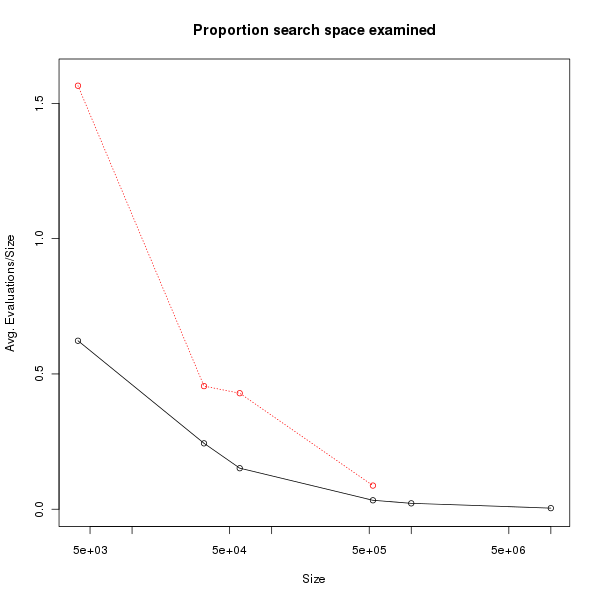
\includegraphics[scale=0.50]{proportion.png}
\caption{Average proportion of search space (that is, number of evaluations divided by search space size)
  vs. search space size for the original Evo++ method (dotted, green or light
  color) and the current Evo10 (dashed, red or intense). Please note
  that the $x$ axis is logarithmic.   \label{fig:prop}}
\end{figure*} 
%
\begin{figure*}[!htb]
\centering
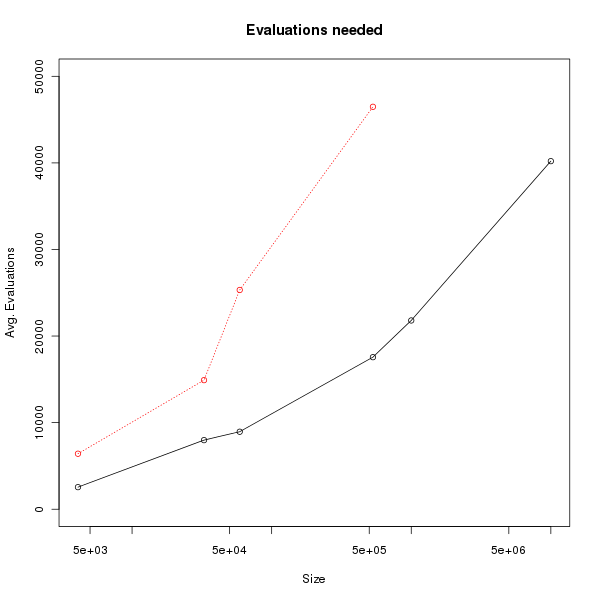
\includegraphics[scale=0.50]{size.png}
\caption{Average number of evaluations 
  vs. search space size for the original Evo++ method (dashed, light
  color) and the current Evo10 (solid, black).  Please note that the
  $x$ axis is logarithmic. \label{fig:size}}
\end{figure*} 
%

As it can be seen in Tables \ref{tab:moves45} and \ref{tab:moves67},
which represent the average number of moves needed to find the
solution, results are quite similar. The average for Evo10 is
consistently higher (more games are needed to find the solution)
but in half the cases the difference is not statistically
significant using Wilcoxon paired test. 
% Antonio - øpuedes poner alguna tablilla con los resultados de
% Wilcoxon? Le darÌa tambiÈn m·s 'cuerpo' al trabajo. :D
% Uf, para quÈ... - JJ
There is a significant
difference for the two smaller sizes ($\ell=4,\kappa=8$ and
$\ell=5,\kappa=8$), but not for the larger sizes  $\ell=5,\kappa=9$
and $\ell=6,7$. This is probably due to the fact that, with increasing
search space size, the difference among 10 and other sample size, even
if they are in different orders of magnitude, become negligible; the
difference between 10\% and 1\% of the actual sample size is
significant, but the difference 0.001\% and 0.0001\% is not. 

However, the difference in the
number of evaluations (shown in Tables  \ref{tab:evals45} and \ref{tab:evals67}), that is, the total population evaluated to find
the solution is quite significant, going from a bit less than half to
a third of the total evaluations for the larger size. This means that
the time needed scales roughly in the same way, but it is even more
interesting to note that it scales better for a fixed size than for
the best consistent set size. Besides, in all cases the algorithm does
not examine the full set of combinations, while previously the number
of combinations evaluated, 6412, was almost 50\% bigger than the search
space size for that problem. The same argument can be applied to the
comparison with Berghman's results (when they are available); Evo++
was able to find solutions which were quite similar to them, but Evo10
obtains an average number of turns that is slightly worse; since we
don't have the complete set of results, and besides they have been
made on a different set of combinations, it is not possible to
compare, but at any rate it would be reasonable to think that this
result is significant. 

 As it can be seen in Figure \ref{fig:prop} the number of evaluations needed to find the solution (which is a bit worse for Evo10) 
% Antonio - yo quitarÌa el admittedly. Hace que el lector repare en
% que Evo10 es peor. Lo mismo si no lo pones, se pasa m·s por alto. :D
% Es que tiene que ser peor, no se usa el conjunto completo - JJ
falls much faster than for Evo++ so that, in fact, we can approach larger sizes than could be done using the previous methods, as the Figure
\ref{fig:size} shows. This figure plots the average number of evaluations needed to find the solution vs. solution size. The most interesting feature of
this plot is the observation that the $\kappa=9,\ell=5$ needs, on
average, as many evaluations as the largest size evaluated here,
$\kappa=10,\ell=7$; however, search space size is 20 times bigger for
this one, which implies that reducing the size of the consistent set
to just ten  multiplies by 20 the size of the search space
approachable using this type of evolutionary algorithms. 

%
\begin{figure}[!h]
\centering
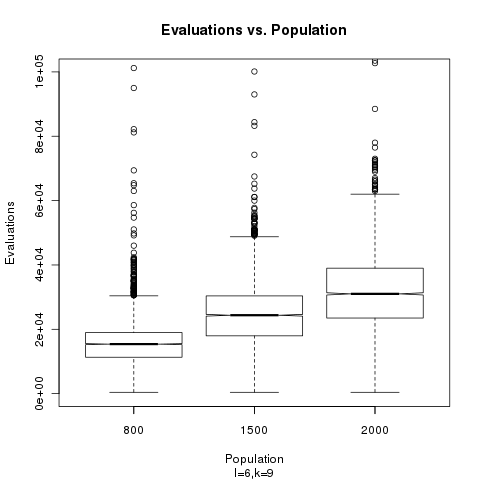
\includegraphics[scale=0.50]{eval-vs-pop.png}
\caption{Boxplot of the average number of evaluations 
  vs. population size for Evo10.  \label{fig:eval:pop}}
\end{figure} 
%
One of the keys of managing to find the solution in less evaluations
is reducing the population size. As a rule of thumb, we have used in
most cases a population that was slightly smaller than the one we used
in Evo++. In evolutionary algorithms, if the population is kept at a
size large enough to maintain diversity, decreasing its size usually
leads to more efficient algorithms. That is why looking at one of the
manageable sizes, $\ell=6, \kappa=9$, we have tested several
population sizes to check its influence on the solutions and the
number of evaluations. These have been plotted in Figure
\ref{fig:eval:pop}, which shows a monotonically increasing number of
evaluations with population size. In fact, the average number of
guesses does not follow a clear trend. It decreases for
population=1500, but it increases for population=2000 to be
approximately the same than for population=800 (in fact, statistically
indistinguishable). This could imply that while population has a
strong influence in the number of evaluations needed to find the
solution, the consistent set size has an influence mainly on the
average number of guesses needed to find the solution. However, a more
precise statistical characterization will need more systematic
experimentation. For the time being, the results obtained show that,
in general, Evo10 needs less or the same population than Evo++ to
obtain similar results using less evaluations and a very similar number of
guesses (at least for the larger search space sizes). 

The experiments performed with the EFE entropy-based method prove that
using a small set size does, in fact, yield good results independently
of the size. In general, it shows also that the smaller size tested
($cs=8$) is never better than Evo10; at most, it is statistically
indistinguishable. However, EFE16 is always better than Evo10, in some
cases statistically so (using Wilcoxon test). This is interesting
since, as indicated in the introduction, every method will need
different $cs$ to obtain good results. In particular, computing
entropy of a set with a small size might produce meaningless results
(while Most Parts will always produce a meaningful result, number of
non-zero partitions); when the size is increased, the results will be
increasingly accurate. In fact, these better results come at the cost
of more evaluations (as should only be expected, since the
evolutionary algorithm must run for a few generations before issuing a
new solution) but, since this implementation is faster than Evo10, it
is in fact noticeably faster: the $\ell=6$ experiments take on average
a single second (while it was from five to 15 seconds for the
non-optimized Evo++ method, depending on $cs$, as shown in the
experiment ChangeLog published below). As usual, raw data, processing scripts and computed results
are available from our GitHub repository
\url{http://github.com/JJ/algorithm-mastermind/experiments/CEC13}. 

\section{Discussion, conclusions and future work}
\label{sec:conclusions}

This paper has shown that using a small and fixed consistent set size
when playing mastermind using evolutionary algorithms does not imply a
deterioration of results, while cutting in half the number of
evaluations needed to find them. This makes the configuration of
the algorithm shown quite suitable for real-time games such as mobile apps
or web games; the actual time varies from less than one second for the
smallest configuration to a few seconds for the whole game in the
biggest configuration shown; the time being roughly proportional to
the number of evaluations, this is at least an improvement of that
order; that is, the time is reduced by 2/3 for the $\kappa=6,\ell=9$
problem, attaining an average of 4.7 seconds, almost one fourth of the
time it can take when we try to achieve the minimum number of turns,
18.6 seconds. This number is closer to the one published by
\cite{Berghman20091880} for this size, 1.284s, although without
running it under the same conditions we cannot be sure. It is in the
same ballpark, anyways. EFE8 and EFE16, since they have been optimized
for speed too, reduce that time even further to an median of 0.74 and
0.92 seconds, respectively (averages are 1.7 and 0.9; in the first
case it is much higher due to the presence of an execution that took
4000 seconds), so that, indeed, we can obtain solutions faster than
the state of the art established by Berghman, and with an average
number of guesses of 6.488 (vs. 6.475) statistically indistinguishable
(p-value = 0.9908); in fact, in this case it is also statistically
indistinguisable from the best value obtained by Evo++ using $cs=100$. 
The time needed to find the solution has a strong
component in the number of evaluations, but it also depends on the
consistent set size, that is why the relation between the time
needed (1/4) is smaller than the relation between number of
evaluations (roughly 1/3, see Table \ref{tab:evals67}) . This allows
also to extend the range of 
feasible sizes, and yields a robust configuration that can be used
throughout any MasterMind problem. 

The explanation for the results obtained in this paper and the small
difference between them and those obtained using a bigger $cs$  (those
computed using Evo++) lies in the fact that the
parameter that sets the size of the consistent set  constitutes just a bound for the actual size the
consistent sets have. This size varies as the turns proceed, as shown in
\cite{DBLP:journals/corr/abs-1207-1315} and go from a considerable
fraction of the total search space to just a few combinations after
several turns have been played. This implies that, in fact, there are
just a few turns or even a single one (which would be the second one, since a fixed
combination is always played on the first turn) in which the evolutionary
algorithm is able to actually find  a number of combinations over the
set limit. At the beginning of the game there are naturally many
combinations, and in fact the evolutionary algorithm only kicks in
when the number of available combinations falls below the set
size. However, once that happens the total size of the consistent set
is smaller than $cs$, which implies that, being impossible to
attain that size, the algorithm stops when the number of consistent
combinations does not increase for three consecutive turns. The fact that the
evolutionary algorithm kicks in after several turns leads also to a
reduction in the number of evaluations needed: only when the
$cs$ falls below 10 new individuals will be generated;
meanwhile, it will be the initial population that will be culled for
consistent combinations after each turn. The number of turns where the
evolutionary algorithm is really working will vary with the problem
size, but it could be as low as one (even 0, in some cases where the
solution is already in the original population and is played). 

%
\begin{figure}[!h]
\centering
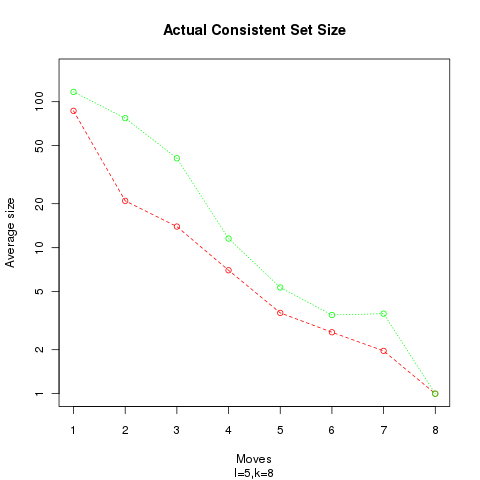
\includegraphics[scale=0.50]{cset-size.png}
\caption{Average actual size of the set of consistent combinations for the original Evo++ method (solid, light
  color) and Evo10 (dashed, intense or red) in the $\ell=5, \kappa=9$ problem.  Please note that the
  $y$ axis is logarithmic. As shown in Table \ref{tab:moves45} the
  bound to the consistent set size was 60 for
  Evo++.  EFE is not shown in this illustration since our objective
  is to prove only that actual consistent set size varies with every
  move, and that changing $cs$ to a smaller value does have an
  influence on that. A similar scenario should be expected for EFE.\label{fig:csize}} 
\end{figure} 
%
The {\em actual} consistent size is
illustrated in Figure \ref{fig:csize}, 
% Antonio - øpor quÈ pones las figuras y tablas tan lejos de donde las
% citas? :D
% JJ cambiada esta 
which shows how the average
(for all 5000 games) size of the consistent set evolves with the turn
number. The actual size of the set depends on the bound; the larger
the bound, the larger the size. In fact, the actual average size is for all
turns, not only for those that are above the limit, which reflects
the fact that this is an {\em average} size and whenever the actual
set size is below the bound the algorithm will work for a few
generations trying to increase the size, until several generations
without improvement have elapsed. This Figure also shows that, for
Evo++, there will be normally 3 turns until the evolutionary algorithm
starts to work (average consistent set size falling below 60), but
Evo10 will produce 4 combinations (including the first one, which is
fixed) before start. Even if this is just a single example of all
problem sizes (and methods) studied in this paper, it is representative in the sense
that the situation will be very similar (Evo10 with smaller consistent
set size than Evo++), although the turns in which the evolutionary
algorithm starts to actually run will vary. 

The fact that the actual consistent set size only falls below $cs$
after a few games (in \ref{fig:csize}, on average, after the third
guess for Evo10 and the first for Evo++)  explains the low number of
evaluations obtained by this new parametrization of the 
algorithm. In fact, many games will be played using the combinations
present in the initial population, with just a few games needing
more than a few generations to find the hidden combination. Please note that,
in the case of the $\ell=6,\kappa=9$ problem, the average number of combinations
played implies that just a few dozens of generations have actually
run; this number obviously increases with the problem size.

As future lines of work, we will try to reduce even more this size and
try to check whether it offers good results for bigger sizes such as
$\ell=7,\kappa=11$ or even $\ell=8,\kappa=12$ and once again try to
beat the state of the art in that size (Berghmat et al. were able to
obtain a solution in less than 9 seconds).  Several consistent set
sizes will be systematically evaluated, looking mainly for a reduction
in the number of evaluations, and time, needed. Eventually, what we
are looking is for a method that is able to resolve problems with
moderate size, but this will need to be tackled from different points
of view: implementation (it always matter, even more so in evolutionary
algorithms \cite{DBLP:conf/iwann/MereloRACML11}), middle-level algorithms
used, even the programming language we will be using. We might even
have to abandon the paradigm of playing always consistent solutions to
settle, sometimes, for non-consistent solutions for the sake of
speed. At these sizes, besides, populations reach a level in which a
concurrent or parallel solution might be a better option to reach the
solution in a reasonable amount of time. 

It is also clear than, when increasing the search space size, the size
of the consistent set will become negligible with respect to the
actual size of the consistent set. This could work both ways: first,
by making the results independent of sample size (for this small size,
at least) or by making the strategy of extracting a sample of a
particular size indistinguishable from finding a single consistent
combination and playing it. As we improve the computation speed, it
would be interesting to take measurements to prove these hypotheses. 

\section*{Acknowledgements}
This work is supported by projects 
TIN2011-28627-C04-02 and TIN2011-28627-C04-01 (ANYSELF), awarded by the Spanish
Ministry of Science and Innovation, P08-TIC-03903 and TIC-6083
(DNEMESIS) awarded by the Andalusian Regional Government, and project
83 (CANUBE) awarded by the CEI-BioTIC UGR
(\url{http://biotic.ugr.es}). 

% trigger a \newpage just before the given reference
% number - used to balance the columns on the last page
% adjust value as needed - may need to be readjusted if
% the document is modified later
%\IEEEtriggeratref{8}
% The "triggered" command can be changed if desired:
%\IEEEtriggercmd{\enlargethispage{-5in}}

% references section

\bibliographystyle{IEEEtran}
%\IEEEtriggeratref{3}
\bibliography{mastermind,geneura,GA-general}

\end{document}


